% Options for packages loaded elsewhere
\PassOptionsToPackage{unicode}{hyperref}
\PassOptionsToPackage{hyphens}{url}
\PassOptionsToPackage{dvipsnames,svgnames,x11names}{xcolor}
%
\documentclass[
  letterpaper,
  DIV=11,
  numbers=noendperiod]{scrreprt}

\usepackage{amsmath,amssymb}
\usepackage{iftex}
\ifPDFTeX
  \usepackage[T1]{fontenc}
  \usepackage[utf8]{inputenc}
  \usepackage{textcomp} % provide euro and other symbols
\else % if luatex or xetex
  \usepackage{unicode-math}
  \defaultfontfeatures{Scale=MatchLowercase}
  \defaultfontfeatures[\rmfamily]{Ligatures=TeX,Scale=1}
\fi
\usepackage{lmodern}
\ifPDFTeX\else  
    % xetex/luatex font selection
\fi
% Use upquote if available, for straight quotes in verbatim environments
\IfFileExists{upquote.sty}{\usepackage{upquote}}{}
\IfFileExists{microtype.sty}{% use microtype if available
  \usepackage[]{microtype}
  \UseMicrotypeSet[protrusion]{basicmath} % disable protrusion for tt fonts
}{}
\makeatletter
\@ifundefined{KOMAClassName}{% if non-KOMA class
  \IfFileExists{parskip.sty}{%
    \usepackage{parskip}
  }{% else
    \setlength{\parindent}{0pt}
    \setlength{\parskip}{6pt plus 2pt minus 1pt}}
}{% if KOMA class
  \KOMAoptions{parskip=half}}
\makeatother
\usepackage{xcolor}
\ifLuaTeX
  \usepackage{luacolor}
  \usepackage[soul]{lua-ul}
\else
  \usepackage{soul}
\fi
\setlength{\emergencystretch}{3em} % prevent overfull lines
\setcounter{secnumdepth}{5}
% Make \paragraph and \subparagraph free-standing
\ifx\paragraph\undefined\else
  \let\oldparagraph\paragraph
  \renewcommand{\paragraph}[1]{\oldparagraph{#1}\mbox{}}
\fi
\ifx\subparagraph\undefined\else
  \let\oldsubparagraph\subparagraph
  \renewcommand{\subparagraph}[1]{\oldsubparagraph{#1}\mbox{}}
\fi


\providecommand{\tightlist}{%
  \setlength{\itemsep}{0pt}\setlength{\parskip}{0pt}}\usepackage{longtable,booktabs,array}
\usepackage{calc} % for calculating minipage widths
% Correct order of tables after \paragraph or \subparagraph
\usepackage{etoolbox}
\makeatletter
\patchcmd\longtable{\par}{\if@noskipsec\mbox{}\fi\par}{}{}
\makeatother
% Allow footnotes in longtable head/foot
\IfFileExists{footnotehyper.sty}{\usepackage{footnotehyper}}{\usepackage{footnote}}
\makesavenoteenv{longtable}
\usepackage{graphicx}
\makeatletter
\def\maxwidth{\ifdim\Gin@nat@width>\linewidth\linewidth\else\Gin@nat@width\fi}
\def\maxheight{\ifdim\Gin@nat@height>\textheight\textheight\else\Gin@nat@height\fi}
\makeatother
% Scale images if necessary, so that they will not overflow the page
% margins by default, and it is still possible to overwrite the defaults
% using explicit options in \includegraphics[width, height, ...]{}
\setkeys{Gin}{width=\maxwidth,height=\maxheight,keepaspectratio}
% Set default figure placement to htbp
\makeatletter
\def\fps@figure{htbp}
\makeatother
\newlength{\cslhangindent}
\setlength{\cslhangindent}{1.5em}
\newlength{\csllabelwidth}
\setlength{\csllabelwidth}{3em}
\newlength{\cslentryspacingunit} % times entry-spacing
\setlength{\cslentryspacingunit}{\parskip}
\newenvironment{CSLReferences}[2] % #1 hanging-ident, #2 entry spacing
 {% don't indent paragraphs
  \setlength{\parindent}{0pt}
  % turn on hanging indent if param 1 is 1
  \ifodd #1
  \let\oldpar\par
  \def\par{\hangindent=\cslhangindent\oldpar}
  \fi
  % set entry spacing
  \setlength{\parskip}{#2\cslentryspacingunit}
 }%
 {}
\usepackage{calc}
\newcommand{\CSLBlock}[1]{#1\hfill\break}
\newcommand{\CSLLeftMargin}[1]{\parbox[t]{\csllabelwidth}{#1}}
\newcommand{\CSLRightInline}[1]{\parbox[t]{\linewidth - \csllabelwidth}{#1}\break}
\newcommand{\CSLIndent}[1]{\hspace{\cslhangindent}#1}

\KOMAoption{captions}{tableheading}
\makeatletter
\@ifpackageloaded{tcolorbox}{}{\usepackage[skins,breakable]{tcolorbox}}
\@ifpackageloaded{fontawesome5}{}{\usepackage{fontawesome5}}
\definecolor{quarto-callout-color}{HTML}{909090}
\definecolor{quarto-callout-note-color}{HTML}{0758E5}
\definecolor{quarto-callout-important-color}{HTML}{CC1914}
\definecolor{quarto-callout-warning-color}{HTML}{EB9113}
\definecolor{quarto-callout-tip-color}{HTML}{00A047}
\definecolor{quarto-callout-caution-color}{HTML}{FC5300}
\definecolor{quarto-callout-color-frame}{HTML}{acacac}
\definecolor{quarto-callout-note-color-frame}{HTML}{4582ec}
\definecolor{quarto-callout-important-color-frame}{HTML}{d9534f}
\definecolor{quarto-callout-warning-color-frame}{HTML}{f0ad4e}
\definecolor{quarto-callout-tip-color-frame}{HTML}{02b875}
\definecolor{quarto-callout-caution-color-frame}{HTML}{fd7e14}
\makeatother
\makeatletter
\makeatother
\makeatletter
\@ifpackageloaded{bookmark}{}{\usepackage{bookmark}}
\makeatother
\makeatletter
\@ifpackageloaded{caption}{}{\usepackage{caption}}
\AtBeginDocument{%
\ifdefined\contentsname
  \renewcommand*\contentsname{Table of contents}
\else
  \newcommand\contentsname{Table of contents}
\fi
\ifdefined\listfigurename
  \renewcommand*\listfigurename{List of Figures}
\else
  \newcommand\listfigurename{List of Figures}
\fi
\ifdefined\listtablename
  \renewcommand*\listtablename{List of Tables}
\else
  \newcommand\listtablename{List of Tables}
\fi
\ifdefined\figurename
  \renewcommand*\figurename{Figure}
\else
  \newcommand\figurename{Figure}
\fi
\ifdefined\tablename
  \renewcommand*\tablename{Table}
\else
  \newcommand\tablename{Table}
\fi
}
\@ifpackageloaded{float}{}{\usepackage{float}}
\floatstyle{ruled}
\@ifundefined{c@chapter}{\newfloat{codelisting}{h}{lop}}{\newfloat{codelisting}{h}{lop}[chapter]}
\floatname{codelisting}{Listing}
\newcommand*\listoflistings{\listof{codelisting}{List of Listings}}
\makeatother
\makeatletter
\@ifpackageloaded{caption}{}{\usepackage{caption}}
\@ifpackageloaded{subcaption}{}{\usepackage{subcaption}}
\makeatother
\makeatletter
\@ifpackageloaded{tcolorbox}{}{\usepackage[skins,breakable]{tcolorbox}}
\makeatother
\makeatletter
\@ifundefined{shadecolor}{\definecolor{shadecolor}{rgb}{.97, .97, .97}}
\makeatother
\makeatletter
\makeatother
\makeatletter
\makeatother
\ifLuaTeX
  \usepackage{selnolig}  % disable illegal ligatures
\fi
\IfFileExists{bookmark.sty}{\usepackage{bookmark}}{\usepackage{hyperref}}
\IfFileExists{xurl.sty}{\usepackage{xurl}}{} % add URL line breaks if available
\urlstyle{same} % disable monospaced font for URLs
\hypersetup{
  pdftitle={The initial 100 papers},
  pdfauthor={Jan-Ru Muller},
  colorlinks=true,
  linkcolor={blue},
  filecolor={Maroon},
  citecolor={Blue},
  urlcolor={Blue},
  pdfcreator={LaTeX via pandoc}}

\title{The initial 100 papers}
\author{Jan-Ru Muller}
\date{2023-06-01}

\begin{document}
\maketitle
\ifdefined\Shaded\renewenvironment{Shaded}{\begin{tcolorbox}[boxrule=0pt, sharp corners, frame hidden, interior hidden, borderline west={3pt}{0pt}{shadecolor}, enhanced, breakable]}{\end{tcolorbox}}\fi

\renewcommand*\contentsname{Table of contents}
{
\hypersetup{linkcolor=}
\setcounter{tocdepth}{2}
\tableofcontents
}
\bookmarksetup{startatroot}

\hypertarget{preface}{%
\chapter*{Preface}\label{preface}}
\addcontentsline{toc}{chapter}{Preface}

\markboth{Preface}{Preface}

This is a Quarto book. It countains x sprints that shall cumulate in the
litreview.

\begin{itemize}
\tightlist
\item
  Include citations count
\item
  Include authors count
\item
  Include affiliations count
\end{itemize}

Document attributes:

\begin{itemize}
\item
  the number of tables is \total{table}
\item
  the number of figures is \total{figure}
\item
  the number of references is \total{citenum}
\item
  add list of tables
\item
  add list of figures
\end{itemize}

\bookmarksetup{startatroot}

\hypertarget{resources}{%
\chapter*{Resources}\label{resources}}
\addcontentsline{toc}{chapter}{Resources}

\markboth{Resources}{Resources}

Over \href{https://www.arthurperret.fr/}{markdown}

\bookmarksetup{startatroot}

\hypertarget{introduction}{%
\chapter{Introduction}\label{introduction}}

This is a book created from markdown and executable code.

See (\textbf{knuth84?}) for additional discussion of literate
programming.

\bookmarksetup{startatroot}

\hypertarget{summary}{%
\chapter{Summary}\label{summary}}

In summary, this book has no content whatsoever.

\part{Part1}

Part 1

\hypertarget{the-first-25-papers}{%
\chapter{The first 25 papers}\label{the-first-25-papers}}

Building a body of knowledge

\hfill\break

Keywords: modelling languages, controlled natural language, extentions,
compliance, MDE

Extract keywords from BOK and create wordcloud. Determine cut-off point
for number of keywords in the header of this article.

I will have the initial 100 articles within 1 month (so on 21 April).
Base myself on NIMS and NEAT. Approach from different angels:

\begin{itemize}
\tightlist
\item
  Accounting, Rulebase, ERP, Compliance (Risk Management)
\item
  Enterprise Achitecture
\end{itemize}

\newpage{}

\begin{center}
``\LaTeX{} uses the \TeX{} typesetting program for formatting
its output, and is itself written in the \TeX{} macro language.
\end{center}

\hypertarget{managing-business-processes-for-regulatory-compliance}{%
\section{Managing business processes for regulatory
compliance}\label{managing-business-processes-for-regulatory-compliance}}

10-03-2023 First step: find three seminal papers published in A star
journals in my field of interest Document search terms for
repeatability. Method: check google scholar for highest rating article
of 10(?) academics that I know off.

Going through my Zotero article listings I came across an article by
\href{https://janvombrocke.com/}{vom Brocke} and 9 co-authors: (vom
Brocke et al. 2021). The article references the Process Mining Manifesto
(\textbf{authority:vanderaalstProcessMiningManifesto2012?}). Based on
the title and year of publication the latter may well qualify as a
seminal paper. The number of listed authors is over 60. It was published
as a conference paper on the The number of reference according to google
scholar per is xxx. It was published in yyy. Wil van der Aalst is an
academic presently associated with Aachen University who, at the time of
the publication worked at Eindhoven University previously used to b

Wil van der Aalst (h score)

Document attributes:

\begin{itemize}
\item
  the number of tablesin this document total
\item
  the number of figures is total
\item
  the number of references is \total{citenum}
\item
  add list of tables
\item
  add list of figures
\end{itemize}

Define h-score Define A star journal Define

\begin{longtable}[]{@{}
  >{\raggedright\arraybackslash}p{(\columnwidth - 16\tabcolsep) * \real{0.0345}}
  >{\raggedright\arraybackslash}p{(\columnwidth - 16\tabcolsep) * \real{0.1034}}
  >{\raggedright\arraybackslash}p{(\columnwidth - 16\tabcolsep) * \real{0.0230}}
  >{\raggedright\arraybackslash}p{(\columnwidth - 16\tabcolsep) * \real{0.0230}}
  >{\raggedright\arraybackslash}p{(\columnwidth - 16\tabcolsep) * \real{0.1609}}
  >{\raggedright\arraybackslash}p{(\columnwidth - 16\tabcolsep) * \real{0.1609}}
  >{\raggedright\arraybackslash}p{(\columnwidth - 16\tabcolsep) * \real{0.1724}}
  >{\raggedright\arraybackslash}p{(\columnwidth - 16\tabcolsep) * \real{0.2069}}
  >{\raggedright\arraybackslash}p{(\columnwidth - 16\tabcolsep) * \real{0.1149}}@{}}
\toprule\noalign{}
\begin{minipage}[b]{\linewidth}\raggedright
\#
\end{minipage} & \begin{minipage}[b]{\linewidth}\raggedright
Article
\end{minipage} & \begin{minipage}[b]{\linewidth}\raggedright
\end{minipage} & \begin{minipage}[b]{\linewidth}\raggedright
\end{minipage} & \begin{minipage}[b]{\linewidth}\raggedright
GSReferences
\end{minipage} & \begin{minipage}[b]{\linewidth}\raggedright
Published in
\end{minipage} & \begin{minipage}[b]{\linewidth}\raggedright
Journal Score
\end{minipage} & \begin{minipage}[b]{\linewidth}\raggedright
Principal Author
\end{minipage} & \begin{minipage}[b]{\linewidth}\raggedright
H-Factor
\end{minipage} \\
\midrule\noalign{}
\endhead
\bottomrule\noalign{}
\endlastfoot
1 & & & & 1 & & & & G - \\
2 & C4 - & & & 2 & & & & G3 - \\
3 & C44 - & & & 3 & & & & G33 - \\
\end{longtable}

\begin{longtable}[]{@{}
  >{\raggedright\arraybackslash}p{(\columnwidth - 16\tabcolsep) * \real{0.0345}}
  >{\raggedright\arraybackslash}p{(\columnwidth - 16\tabcolsep) * \real{0.1034}}
  >{\raggedright\arraybackslash}p{(\columnwidth - 16\tabcolsep) * \real{0.0230}}
  >{\raggedright\arraybackslash}p{(\columnwidth - 16\tabcolsep) * \real{0.0230}}
  >{\raggedright\arraybackslash}p{(\columnwidth - 16\tabcolsep) * \real{0.1609}}
  >{\raggedright\arraybackslash}p{(\columnwidth - 16\tabcolsep) * \real{0.1609}}
  >{\raggedright\arraybackslash}p{(\columnwidth - 16\tabcolsep) * \real{0.1724}}
  >{\raggedright\arraybackslash}p{(\columnwidth - 16\tabcolsep) * \real{0.2069}}
  >{\raggedright\arraybackslash}p{(\columnwidth - 16\tabcolsep) * \real{0.1149}}@{}}
\toprule\noalign{}
\begin{minipage}[b]{\linewidth}\raggedright
\#
\end{minipage} & \begin{minipage}[b]{\linewidth}\raggedright
Article
\end{minipage} & \begin{minipage}[b]{\linewidth}\raggedright
\end{minipage} & \begin{minipage}[b]{\linewidth}\raggedright
\end{minipage} & \begin{minipage}[b]{\linewidth}\raggedright
GSReferences
\end{minipage} & \begin{minipage}[b]{\linewidth}\raggedright
Published in
\end{minipage} & \begin{minipage}[b]{\linewidth}\raggedright
Journal Score
\end{minipage} & \begin{minipage}[b]{\linewidth}\raggedright
Principal Author
\end{minipage} & \begin{minipage}[b]{\linewidth}\raggedright
H-Factor
\end{minipage} \\
\midrule\noalign{}
\endhead
\bottomrule\noalign{}
\endlastfoot
\end{longtable}

\hypertarget{day01-whatever-happened}{%
\section{{[}18-03-2023 / day01{]} Whatever
happened}\label{day01-whatever-happened}}

Whatever happened to the 60 authors \ldots{}

Continuation of: ``Whatever happened to the class of 2021'' (Process
Mining Manifesto)

\hypertarget{day02-the-italian-connection}{%
\section{{[}19-03-2023 / day02{]} The Italian
connection}\label{day02-the-italian-connection}}

Guido Governatori is an italian who completed his PhD in Legal
Informatics in 1997. Since he moved to Queensland University of
Technology in Australia.

One of his papers with Sadiq is about checking between business
processes and business contracts (Governatori, Milosevic, and Sadiq
2006) - 366 citations on google scholar. Sadiq and Governatori also
wrote together about modelling controls objectives for business process
compliance (Sadiq, Governatori, and Namiri 2007) - 615 citations.

Guido
Governatori\index[authors]{Governatori, Guido \orcidlink{https://orcid.org/0000-0002-9878-2762}}
and Shazia Sadiq then wrote (Sadiq and Governatori 2010) together - 148
citations.

Governatori and
Sadiq\index[authors]{Sadiq, Shazia \orcidlink{https://orcid.org/0000-0001-6739-4145}}
often appear as co-authors on papers (query string WoS and query result
count). Was Lu a PhD student with Governatori?

To find the number of publications they both worked on I may want to
look into \href{https://www.bibliometrix.org/home/}{bibliometrix}: a R
tool for comprehensive bibliometric analysis of scientific literature.
This is in R, there maybe similar tools for Python. Pybibliometrics
\href{}{} looks to be an interface to Elsevier Scopus only.

\hypertarget{day03-literature-graph-database}{%
\section{{[}20-03-2023 / day03{]} Literature (graph)
database}\label{day03-literature-graph-database}}

Two ideas that I will have to explore further:

\begin{itemize}
\item
  Building a small application to maintain a graph database (outside
  Zotero) for linking articles. Also see
  \href{https://realpython.com/python-django-blog}{Build a Blog Using
  Django, Vue and GraphQL}
\item
  Building `something' to discover a literature gap. Also see
  \href{https://pubmed.ncbi.nlm.nih.gov/26262393/}{Constructing a Graph
  Database for Semantic Literature-Based Discovery}
\end{itemize}

In any case scan all bibliometrics packages on github
\href{https://github.com/topics/bibliometrics}{bibliometrics}, for
example \href{https://github.com/NLeSC/litstudy}{LitStudy} from the NL
escience institute in Amsterdam.

The purpose of the first will be to facilitate interaction with the
literature. For example, easily being able to extract research methods
or dataset descriptions. Ref. article abstract template that was sent to
me by Imre.

\hypertarget{day04-quick-and-dirty}{%
\section{{[}21-03-2024 / day04{]} Quick and
dirty}\label{day04-quick-and-dirty}}

In a recent paper (2021) vom
Brocke\index[authors]{Brocke, Jan Vom \orcidlink{https://orcid.org/0000-0002-0071-3719}}
, van der
Aalst\index[authors]{Aalst, Wil van der \orcidlink{https://orcid.org/0000-0002-0955-6940}}
and 8 co-authors propose Process science as a separate discipline
\href{https://papers.ssrn.com/sol3/papers.cfm?abstract_id=3916817}{Process
Science: The Interdisciplinary Study of Continuous Change}

Maybe add BPMN Extentions:

\begin{itemize}
\item
  BPMN-L: A BPMN extension for modeling of process
  landscapes\index{Landscapes} (Polančič 2020) - \textbf{7} citations.
  The paper is by Gregor
  Polančič\index[authors]{Polančič, Gregor \orcidlink{https://orcid.org/0000-0002-4746-1010}}
  whose \href{https://polancic.com/}{blog} I follow.
\item
  BPMS-RA: a novel reference architecture for business process
  management systems (Pourmirza et al. 2019) - \textbf{13} citations.
\item
  BPMN extention for Risk Handling (Marcinkowski and Kuciapski 2012) -
  \textbf{44} citations.
\end{itemize}

\hypertarget{day05-vscode-online-to-the-rescue}{%
\section{\texorpdfstring{{[}22-03-2023 / day05{]} VSCode online \st{to
the
rescue}}{{[}22-03-2023 / day05{]} VSCode online to the rescue}}\label{day05-vscode-online-to-the-rescue}}

\begin{itemize}
\item
  A Controlled Natural Language for Financial Services Compliance
  Checking (Azzopardi, Colombo, and Pace 2018) - \textbf{7} citations.
  Seems to be right on my subject but only (very) few citations. The
  abbreviation for Controlled Natural Language is CNL\index{CNL}
\item
  El Kharbili\index[authors]{El Kharbili, Marwane} - 2012 - Business
  process regulatory compliance management (El Kharbili 2012)
  \textbf{96} citations. Affiliation University of Luxemburg
\item
  Separating compliance management and business process management
  (Ramezani et al. 2011) - \textbf{59} citations, written by Dirk
  Fahland
  \index[authors]{Fahland, Dirk \orcidlink{https://orcid.org/0000-0002-1993-9363}},
  Elham Ramezani\index[authors]{Ramezani, Elham}, Jan Martijn van der
  Werf\index[authors]{Werf, Jan Martijn van der \orcidlink{https://orcid.org/0000-0002-7264-381X}}
  and Peter Mattheis\index[authors]{Mattheis, Peter}.
\end{itemize}

\hypertarget{day06-foundational-books}{%
\section{{[}23-03-2023 / day06{]} Foundational
Books?}\label{day06-foundational-books}}

\begin{tcolorbox}[enhanced jigsaw, opacityback=0, rightrule=.15mm, colbacktitle=quarto-callout-tip-color!10!white, coltitle=black, leftrule=.75mm, titlerule=0mm, toptitle=1mm, colframe=quarto-callout-tip-color-frame, colback=white, breakable, bottomtitle=1mm, bottomrule=.15mm, arc=.35mm, title=\textcolor{quarto-callout-tip-color}{\faLightbulb}\hspace{0.5em}{\href{https://bpt.hpi.uni-potsdam.de/people/mathias-weske/}{Mathias
Weske, Universität Potsdam}}, opacitybacktitle=0.6, toprule=.15mm, left=2mm]

\index[authors]{Weske, Mathias \orcidlink{https://orcid.org/0000-0002-3346-2442}}

Business process management architectures (Weske 2007) - \textbf{4775}
citations

\end{tcolorbox}

\begin{tcolorbox}[enhanced jigsaw, opacityback=0, rightrule=.15mm, colbacktitle=quarto-callout-tip-color!10!white, coltitle=black, leftrule=.75mm, titlerule=0mm, toptitle=1mm, colframe=quarto-callout-tip-color-frame, colback=white, breakable, bottomtitle=1mm, bottomrule=.15mm, arc=.35mm, title=\textcolor{quarto-callout-tip-color}{\faLightbulb}\hspace{0.5em}{\href{https://kodu.ut.ee/~dumas/}{Marlon Dumas, University of Tartu}}, opacitybacktitle=0.6, toprule=.15mm, left=2mm]

\index[authors]{Dumas, Marlon \orcidlink{https://orcid.org/0000-0002-9247-7476}}

Fundamentals of business process management (Dumas et al. 2013) -
\textbf{3391} citations

\end{tcolorbox}

Process Mining: a research agenda by
\href{https://orcid.org/0000-0002-0955-6940}{Van der Aalst} and Weijters
(2004:863)

And now: Process Science (vom Brocke et al. 2021)

\hypertarget{day07-literature-reviews}{%
\section{{[}24-03-2023 / day07{]} Literature
Reviews}\label{day07-literature-reviews}}

Samples of literature reviews (and what I think about them)

\begin{itemize}
\item
  Business Process Management and Digital Innovations: A Systematic
  Literature Review (Ahmad and Van Looy 2020) (SLR\index{SLR}) by Amy
  Van Looy and Tahir Ahmad
  \index[authors]{Ahmad, Tahir \orcidlink{https://orcid.org/0000-0003-0765-7059}}
\item
  (Moreno-Montes de Oca et al. 2015) now lives and works in Cuba?
\end{itemize}

\hypertarget{day08-methodologies}{%
\section{{[}25-03-2023 / day08{]}
Methodologies}\label{day08-methodologies}}

Now add three articles where I write about the (research) methodology
used.

\begin{itemize}
\tightlist
\item
  (Häußler, Esser, and Borrmann 2021) not about methodology but
  interesting model interaction BIM, XBRL\index{XBRL},
\end{itemize}

\hypertarget{day09-the-gap}{%
\section{{[}29-03-2023 / day09{]} The GAP}\label{day09-the-gap}}

Articles mentioning GAP's:

\begin{itemize}
\tightlist
\item
  This is about modelling concepts for internal controls
  (BPMN\index{BPMN} extention)(Schultz and Radloff 2014) - ?? citations
\end{itemize}

Stijn
Hoppenbrouwers\index[authors]{Hoppenbrouwers, Stijn \orcidlink{https://orcid.org/0000-0002-1137-2999}}
(HAN)

Thesis: (Hoppenbrouwers 2003)

Hajo Reijers Utrechte University in an article about the role of
blockchain (Mendling et al. 2018). Note: there are 32(!) authors listed
in this paper.

\hypertarget{day10-vlerick}{%
\section{{[}30-03-2023 / day10{]} Vlerick}\label{day10-vlerick}}

Three inspiring papers by Stijn
Viaene\index[authors]{Viaene, Stijn \orcidlink{https://orcid.org/0000-0002-1600-4706}}

\begin{itemize}
\tightlist
\item
  Ten principles of (vom Brocke et al. 2014) - \textbf{405} citations.
  This paper was co-authored with vom
  Brocke\index[authors]{Brocke, Jan Vom \orcidlink{https://orcid.org/0000-0002-0071-3719}}
  University of Liechtenstein
\end{itemize}

Three inspiring papers by \href{https://www.amyvanlooy.eu/home}{Amy Van
Looy}\index[authors]{Looy, Amy Van \orcidlink{https://orcid.org/0000-0002-7992-1528}}\footnote{Ghent
  University: Ghent, BE}

\begin{itemize}
\tightlist
\item
  BPO Configuration Taxonomy (Van Looy, Clarysse, and Trkman 2021)
\end{itemize}

Ook beschrijven waarom inspiring \ldots{}

\begin{itemize}
\tightlist
\item
  Design science research on Developing a toof for process-oriented
  appraisals and rewards (Shafagatova and Van Looy 2021) written with
  Aygun
  Shafagatova\index[authors]{Shafagatova, Aygun \orcidlink{https://orcid.org/0000-0001-9837-4585}}
  who obtained her PhD in 2021 and is currently with EY in Gent.
\end{itemize}

\hypertarget{day11-mieke-jans2}{%
\section[{[}31-03-2023 / day11{]} Mieke
Jans]{\texorpdfstring{{[}31-03-2023 / day11{]} Mieke
Jans\footnote{Universiteit Hasselt: Hasselt, Limburg, BE}}{{[}31-03-2023 / day11{]} Mieke Jans}}\label{day11-mieke-jans2}}

\index[authors]{Jans, Mieke \orcidlink{https://orcid.org/0000-0002-9171-2403}}

Continuous auditing(Jans and Hosseinpour 2019) - \textbf{38} citations.

\hypertarget{day12-matthias-trier}{%
\section{{[}31-03-2023 / day12{]} Matthias
Trier}\label{day12-matthias-trier}}

Bij alle professors ook een linkje naar hun scopus profiel (met logo)

\index[authors]{Trier, Matthias \orcidlink{https://orcid.org/0000-0002-8758-2968}}

Matthias Trief

Visiting researcher, Copenhagen Business School, Department of
Digitalization

\hypertarget{day13-monique-snoeck3}{%
\section[{[}31-03-2023 / day13{]} Monique
Snoeck]{\texorpdfstring{{[}31-03-2023 / day13{]} Monique
Snoeck\footnote{KU Leuven: Leuven, BE}}{{[}31-03-2023 / day13{]} Monique Snoeck}}\label{day13-monique-snoeck3}}

\index[authors]{Snoeck, Monique \orcidlink{https://orcid.org/0000-0002-3824-3214}}

Monique Snoeck

Wim Laurier (person having experience with Merode)

\index[authors]{Laurier, Wim \orcidlink{https://orcid.org/0000-0002-9448-248X}}

(linked met Stijn)

Jochen De Weerdt (co-author of Monique Snoeck)

\index[authors]{De Weerdt, Jochen \orcidlink{https://orcid.org/0000-0001-6151-0504}}

h-index(all): 32

Amy Van
Looy\index[authors]{Looy, Amy Van \orcidlink{https://orcid.org/0000-0002-7992-1528}},
with Isel Moreno-Montes de
Oca\index[authors]{Moreno-Montes de Oca, Isel \orcidlink{https://orcid.org/0000-0001-5288-5654}}
who is currently Professor in Cuba (Moreno-Montes de Oca et al. 2015)

Dijkman\index[authors]{Dijkman, Remco \orcidlink{https://orcid.org/0000-0003-4083-0036}}
TUE

Proper, H. A https://www.springer.com/series/8371/books?page=2

\hypertarget{day14-geert-poels4}{%
\section[{[}01-04-2023 / day14{]} Geert
Poels]{\texorpdfstring{{[}01-04-2023 / day14{]} Geert
Poels\footnote{Universiteit Gent: Gent, BE}}{{[}01-04-2023 / day14{]} Geert Poels}}\label{day14-geert-poels4}}

\index[authors]{Poels, Geert \orcidlink{https://orcid.org/0000-0001-9247-6150}}

4644 citations

\hypertarget{day15-michael-werner5}{%
\section[{[}02-04-2023 / day15{]} Michael
Werner]{\texorpdfstring{{[}02-04-2023 / day15{]} Michael
Werner\footnote{Universiteit van Amsterdam: Amsterdam, NL}}{{[}02-04-2023 / day15{]} Michael Werner}}\label{day15-michael-werner5}}

Person(s) with SAP access

\index[authors]{Werner, Michael \orcidlink{https://orcid.org/0000-0002-3036-1478}}

Michael Werner

m.werner@uva.nl

See Figure~\ref{fig-authors} for most cited authors.

See Figure~\ref{fig-sources} for most cited sources.

\hypertarget{day16-jan-recker}{%
\section{{[}04-04-2023 / day16{]} Jan Recker}\label{day16-jan-recker}}

Jan Recker

\index[authors]{Recker, Jan \orcidlink{https://orcid.org/0000-0002-2072-5792}}

\hypertarget{day17-jan-mendling}{%
\section{{[}06-04-2023 / day17{]} Jan
Mendling}\label{day17-jan-mendling}}

\index[authors]{Mendling, Jan \orcidlink{https://orcid.org/0000-0002-7260-524X}}

Building a complementary agenda for business process management and
digital innovation. (Mendling, Pentland, and Recker 2020) - 101
citations.

\newpage{}

\hypertarget{most-relevant-authors-sources}{%
\section{Most Relevant Authors \&
Sources}\label{most-relevant-authors-sources}}

{concept}

\begin{figure}

{\centering 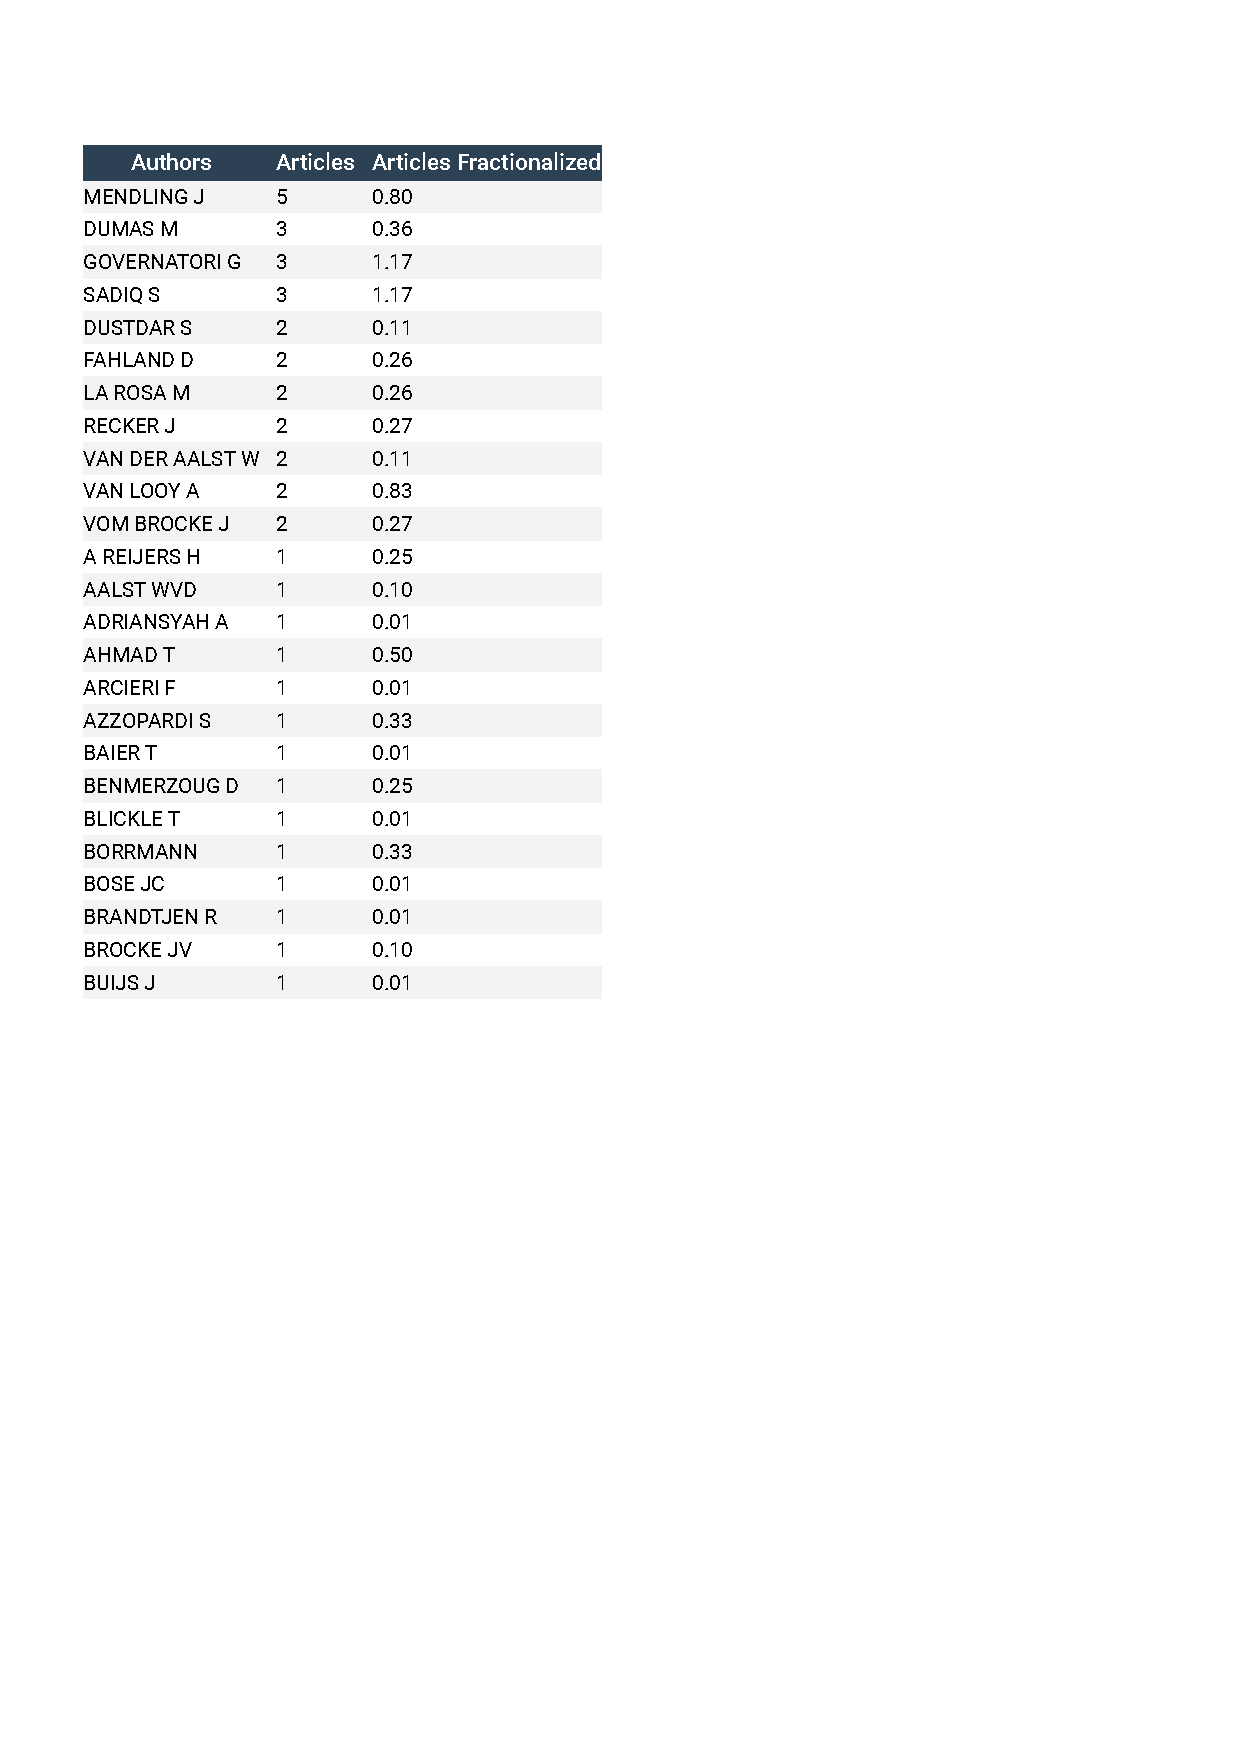
\includegraphics{./static/Most_Relevant_Authors.pdf}

}

\caption{\label{fig-authors}Most relevant authors}

\end{figure}

\begin{figure}

{\centering 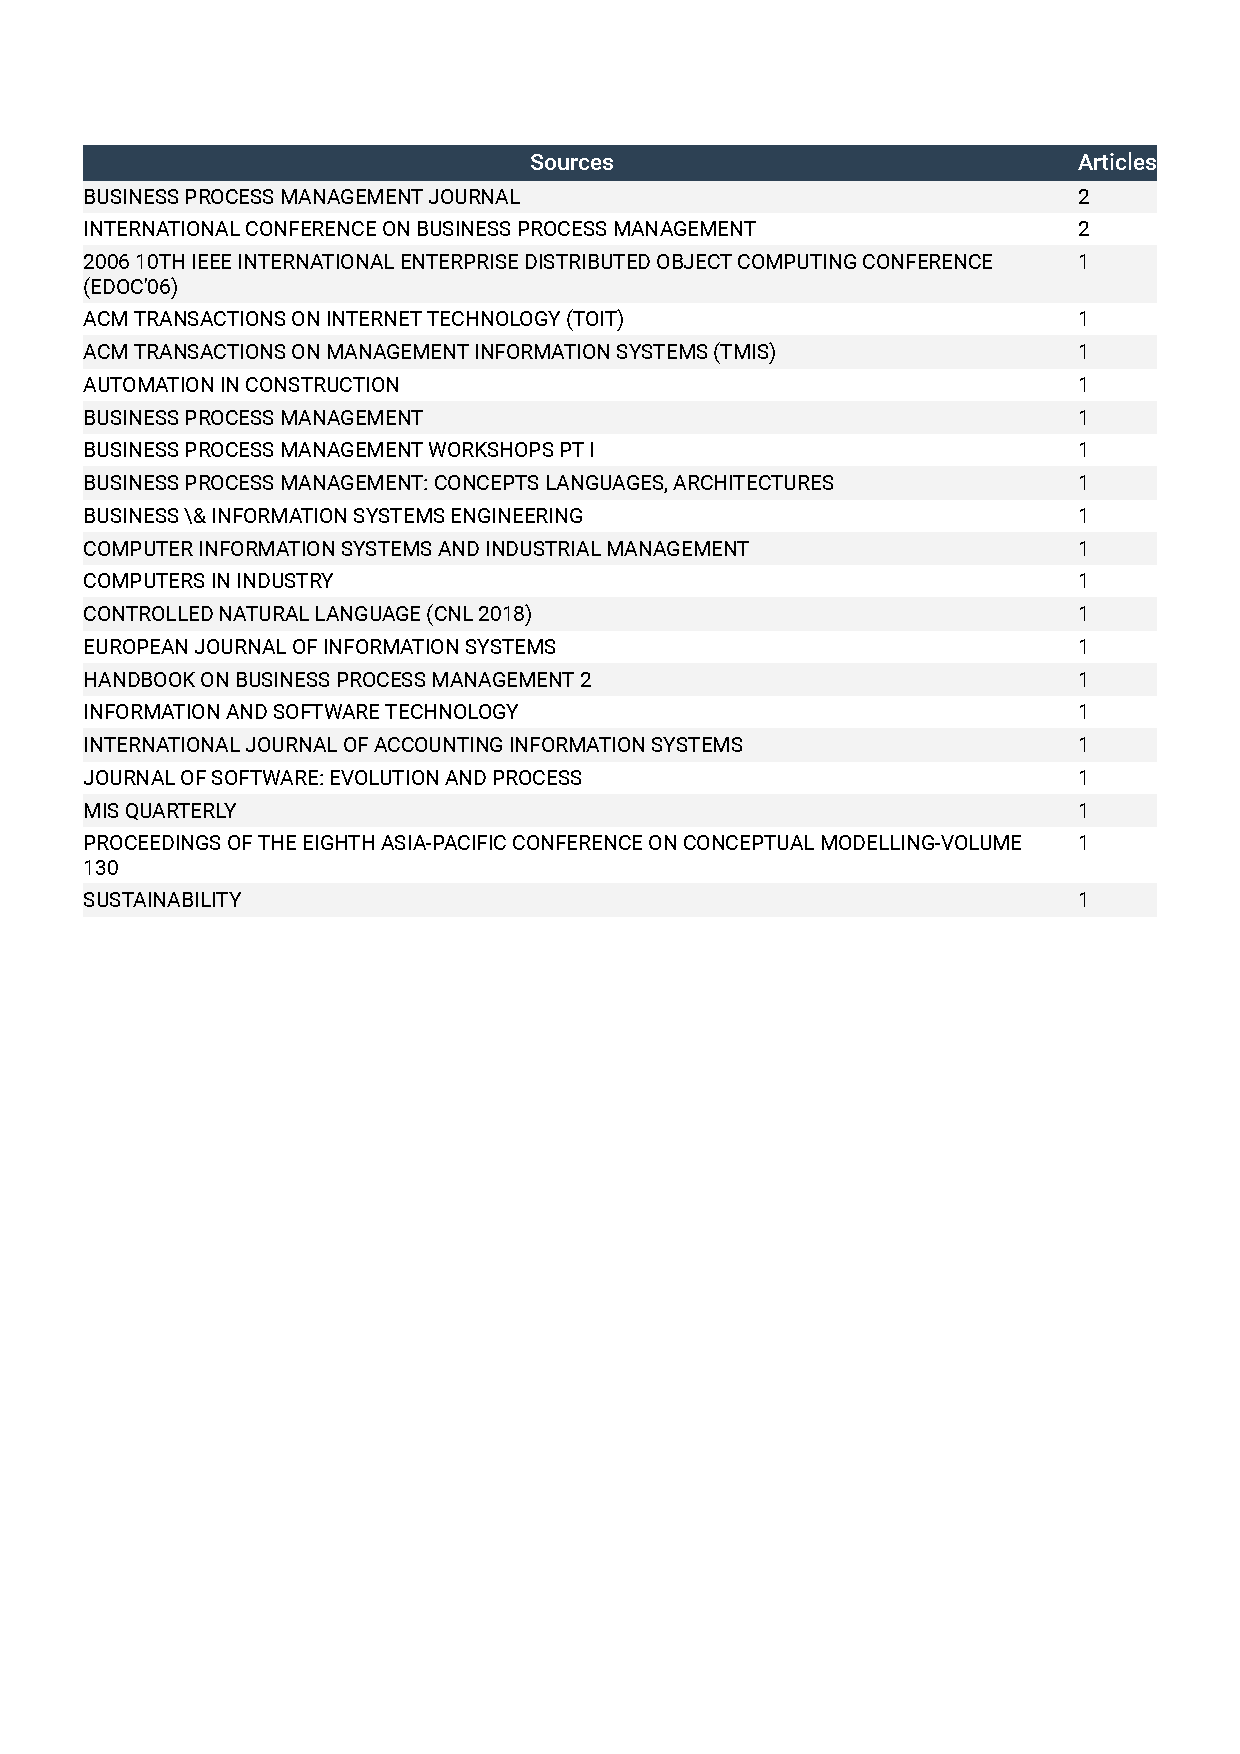
\includegraphics{./static/Most_Relevant_Sources.pdf}

}

\caption{\label{fig-sources}Most relevant sources}

\end{figure}

\newpage{}

\hypertarget{works-cited-25}{%
\section{Works Cited (25)}\label{works-cited-25}}

\hypertarget{software-support}{%
\chapter{Software Support}\label{software-support}}

\hypertarget{tools}{%
\section{{[}27-05-2023{]} Tools}\label{tools}}

(https://pypi.org/project/refextract/)

(https://docs.readme.com/rdmd/docs/getting-started)

ORCID toegevoegd aan de authors index using the latex package
``orcidlink''.

Idea for backlog: obtain keywords via orcid api (python) and build
wordcloud.

\hypertarget{day08-include-academicons}{%
\section{{[}26-05-2024 / day08{]} Include
Academicons}\label{day08-include-academicons}}

\href{https://schochastics.quarto.pub/academicons-quarto-extension/}{quarto
extention}

Potentially add google scholar link to author index

Possibly also use
\href{https://www.w3schools.com/icons/fontawesome5_icons_computers.asp}{fontawesome
computer icons}

Look into
\href{https://shafayetshafee.github.io/interactive-sql/example.html}{interactive-sql}
which may help to clarify relationships between accounts and
``verdichtingen''. Note that interactive-sql is a wrapper aroung
\href{https://sqlime.org/about.html}{sqlime}.

\hypertarget{document-attributes}{%
\section{Document attributes}\label{document-attributes}}

Current thinking: use latex package

\begin{itemize}
\item
  \totcounter
\item
  \regtotcounter{table}
\item
  \regtotcounter{figure}
\end{itemize}

In case of output to html, and not to loose functionality of certain
latex packages (such as orcid):

\begin{itemize}
\tightlist
\item
  Document is processed and variables obtain a number.
\item
  Intermediary file is saved.
\item
  Variables are read
  \href{https://tex.stackexchange.com/questions/321346/how-to-read-a-variable-from-a-file-in-latex}{ref.
  texexchange}
\item
  html snippet creation \href{https://texfaq.org/FAQ-LaTeX2HTML}{html
  snippet}
\item
  html snippet is included in header, footer, or body of file
\end{itemize}

\hypertarget{references}{%
\chapter*{References}\label{references}}
\addcontentsline{toc}{chapter}{References}

\markboth{References}{References}

\hypertarget{refs}{}
\begin{CSLReferences}{1}{0}
\leavevmode\vadjust pre{\hypertarget{ref-ahmadBusinessProcessManagement2020}{}}%
Ahmad, Tahir, and Amy Van Looy. 2020. {``Business {Process Management}
and {Digital Innovations}: {A Systematic Literature Review}.''}
\emph{Sustainability} 12 (17): 6827.
\url{https://doi.org/10.3390/su12176827}.

\leavevmode\vadjust pre{\hypertarget{ref-WOS:000467454700002}{}}%
Azzopardi, Shaun, Christian Colombo, and Gordon J. Pace. 2018. {``A
Controlled Natural Language for Financial Services Compliance
Checking.''} Proceedings Paper. In \emph{{CONTROLLED NATURAL LANGUAGE}
({CNL} 2018)}, edited by B Davis, CM Keet, and A Wyner, 304:11--20.
Frontiers in Artificial Intelligence and Applications. {NIEUWE HEMWEG
6B, 1013 BG AMSTERDAM, NETHERLANDS}: {IOS PRESS}.
\url{https://doi.org/10.3233/978-1-61499-904-1-11}.

\leavevmode\vadjust pre{\hypertarget{ref-dumasFundamentalsBusinessProcess2013}{}}%
Dumas, Marlon, Marcello La Rosa, Jan Mendling, and Hajo A Reijers. 2013.
\emph{Fundamentals of Business Process Management}. {Springer}.

\leavevmode\vadjust pre{\hypertarget{ref-elkharbiliBusinessProcessRegulatory2012}{}}%
El Kharbili, Marwane. 2012. {``Business Process Regulatory Compliance
Management Solution Frameworks: {A} Comparative Evaluation.''}
Proceedings Paper. In \emph{Proceedings of the {Eighth Asia-Pacific
Conference} on {Conceptual Modelling-Volume} 130}, 23--32.

\leavevmode\vadjust pre{\hypertarget{ref-governatoriComplianceCheckingBusiness2006}{}}%
Governatori, Guido, Zoran Milosevic, and Shazia Sadiq. 2006.
{``Compliance Checking Between Business Processes and Business
Contracts.''} Proceedings Paper. In \emph{2006 10th {IEEE International
Enterprise Distributed Object Computing Conference} ({EDOC}'06)},
221--32. {IEEE}.

\leavevmode\vadjust pre{\hypertarget{ref-hausslerCodeComplianceChecking2021}{}}%
Häußler, Marco, Sebastian Esser, and André Borrmann. 2021. {``Code
Compliance Checking of Railway Designs by Integrating {BIM}, {BPMN} and
{DMN}.''} Journal Article. \emph{Automation in Construction} 121
(January): 103427. \url{https://doi.org/10.1016/j.autcon.2020.103427}.

\leavevmode\vadjust pre{\hypertarget{ref-hoppenbrouwersFreezingLanguageConceptualisation2003}{}}%
Hoppenbrouwers, Stijn Johannes Baptist Apollonia. 2003. \emph{Freezing
Language: Conceptualisation Processes Across {ICT-supported}
Organisations}. {{[}Sl: sn{]}}.

\leavevmode\vadjust pre{\hypertarget{ref-jansHowActiveLearning2019}{}}%
Jans, Mieke, and Marzie Hosseinpour. 2019. {``How Active Learning and
Process Mining Can Act as {Continuous Auditing} Catalyst.''} Journal
\{\{Article\}\}. \emph{International Journal of Accounting Information
Systems} 32: 44--58. \url{https://doi.org/10.1016/j.accinf.2018.11.002}.

\leavevmode\vadjust pre{\hypertarget{ref-marcinkowskiBusinessProcessModeling2012}{}}%
Marcinkowski, Bartosz, and Michal Kuciapski. 2012. {``A {Business
Process Modeling Notation Extension} for {Risk Handling}.''} In
\emph{Computer {Information Systems} and {Industrial Management}},
edited by David Hutchison, Takeo Kanade, Josef Kittler, Jon M.
Kleinberg, Friedemann Mattern, John C. Mitchell, Moni Naor, et al.,
7564:374--81. {Berlin, Heidelberg}: {Springer Berlin Heidelberg}.
\url{https://doi.org/10.1007/978-3-642-33260-9_32}.

\leavevmode\vadjust pre{\hypertarget{ref-mendlingBuildingComplementaryAgenda2020}{}}%
Mendling, Jan, Brian T. Pentland, and Jan Recker. 2020. {``Building a
Complementary Agenda for Business Process Management and Digital
Innovation.''} \emph{European Journal of Information Systems} 29 (3):
208--19. \url{https://doi.org/10.1080/0960085X.2020.1755207}.

\leavevmode\vadjust pre{\hypertarget{ref-mendlingBlockchainsBusinessProcess2018}{}}%
Mendling, Jan, Ingo Weber, Wil Van Der Aalst, Jan Vom Brocke, Cristina
Cabanillas, Florian Daniel, Søren Debois, Claudio Di Ciccio, Marlon
Dumas, and Schahram Dustdar. 2018. {``Blockchains for Business Process
Management-Challenges and Opportunities.''} \emph{ACM Transactions on
Management Information Systems (TMIS)} 9 (1): 1--16.

\leavevmode\vadjust pre{\hypertarget{ref-moreno-montesdeocaSystematicLiteratureReview2015}{}}%
Moreno-Montes de Oca, Isel, Monique Snoeck, Hajo A. Reijers, and Abel
Rodríguez-Morffi. 2015. {``A Systematic Literature Review of Studies on
Business Process Modeling Quality.''} \emph{Information and Software
Technology} 58 (February): 187--205.
\url{https://doi.org/10.1016/j.infsof.2014.07.011}.

\leavevmode\vadjust pre{\hypertarget{ref-polancicBPMNLBPMNExtension2020}{}}%
Polančič, Gregor. 2020. {``{BPMN-L}: {A BPMN} Extension for Modeling of
Process Landscapes.''} \emph{Computers in Industry} 121: 103276.

\leavevmode\vadjust pre{\hypertarget{ref-pourmirzaBPMSRANovelReference2019}{}}%
Pourmirza, Shaya, Sander Peters, Remco Dijkman, and Paul Grefen. 2019.
{``{BPMS-RA}: A Novel Reference Architecture for Business Process
Management Systems.''} \emph{ACM Transactions on Internet Technology
(TOIT)} 19 (1): 1--23.

\leavevmode\vadjust pre{\hypertarget{ref-ramezaniSeparatingComplianceManagement2011}{}}%
Ramezani, Elham, Dirk Fahland, Jan Martijn van der Werf, and Peter
Mattheis. 2011. {``Separating Compliance Management and Business Process
Management.''} In \emph{International {Conference} on {Business Process
Management}}, 459--64. {Springer}.

\leavevmode\vadjust pre{\hypertarget{ref-sadiqManagingRegulatoryCompliance2010}{}}%
Sadiq, Shazia, and Guido Governatori. 2010. {``Managing {Regulatory
Compliance} in {Business Processes}.''} In \emph{Handbook on {Business
Process Management} 2}, edited by Jan vom Brocke and Michael Rosemann,
159--75. {Berlin, Heidelberg}: {Springer Berlin Heidelberg}.
\url{https://doi.org/10.1007/978-3-642-01982-1_8}.

\leavevmode\vadjust pre{\hypertarget{ref-sadiqModelingControlObjectives2007}{}}%
Sadiq, Shazia, Guido Governatori, and Kioumars Namiri. 2007. {``Modeling
Control Objectives for Business Process Compliance.''} In
\emph{International Conference on Business Process Management}, 149--64.
{Springer}.

\leavevmode\vadjust pre{\hypertarget{ref-schultzModelingConceptsInternal2014}{}}%
Schultz, Martin, and Michael Radloff. 2014. {``Modeling {Concepts} for
{Internal Controls} in {Business Processes} \textendash{} {An
Empirically Grounded Extension} of {BPMN}.''} In \emph{Business {Process
Management}}, edited by Shazia Sadiq, Pnina Soffer, and Hagen Völzer,
8659:184--99. {Cham}: {Springer International Publishing}.
\url{https://doi.org/10.1007/978-3-319-10172-9_12}.

\leavevmode\vadjust pre{\hypertarget{ref-shafagatovaDevelopingToolProcess2021}{}}%
Shafagatova, Aygun, and Amy Van Looy. 2021. {``Developing a Tool for
Process-Oriented Appraisals and Rewards: {Design} Science Research.''}
\emph{Journal of Software: Evolution and Process} 33 (3): e2321.

\leavevmode\vadjust pre{\hypertarget{ref-vanlooyConfigurationTaxonomyBusiness2021}{}}%
Van Looy, Amy, Els Clarysse, and Peter Trkman. 2021. {``A {Configuration
Taxonomy} of {Business Process Orientation}.''} \emph{Business \&
Information Systems Engineering}, May, In press.
\url{https://doi.org/10.1007/s12599-021-00700-4}.

\leavevmode\vadjust pre{\hypertarget{ref-vombrockeTenPrinciplesGood2014}{}}%
vom Brocke, Jan, Theresa Schmiedel, Jan Recker, Peter Trkman, Willem
Mertens, and Stijn Viaene. 2014. {``Ten Principles of Good Business
Process Management.''} Edited by Dr Thomas Kohlborn Professor Jens
Poeppelbuss and Dr Maximilian Roeglinger. \emph{Business Process
Management Journal} 20 (4): 530--48.
\url{https://doi.org/10.1108/BPMJ-06-2013-0074}.

\leavevmode\vadjust pre{\hypertarget{ref-vombrockeProcessScienceInterdisciplinary2021}{}}%
vom Brocke, Jan, Wil van der Aalst, Thomas Grisold, Waldemar Kremser,
Jan Mendling, Brian Pentland, Jan Recker, Maximilian Roeglinger, Michael
Rosemann, and Barbara Weber. 2021. {``Process {Science}: {The
Interdisciplinary Study} of {Continuous Change}.''} \{\{SSRN Scholarly
Paper\}\}. {Rochester, NY}. \url{https://doi.org/10.2139/ssrn.3916817}.

\leavevmode\vadjust pre{\hypertarget{ref-Weske2007}{}}%
Weske, Mathias. 2007. {``Business Process Management Architectures.''}
In \emph{Business Process Management: {Concepts}, Languages,
Architectures}, 305--43. {Berlin, Heidelberg}: {Springer Berlin
Heidelberg}. \url{https://doi.org/10.1007/978-3-540-73522-9_7}.

\end{CSLReferences}

\hypertarget{authors}{%
\chapter*{Authors}\label{authors}}
\addcontentsline{toc}{chapter}{Authors}

\markboth{Authors}{Authors}

\cleardoublepage
\phantomsection
\addcontentsline{toc}{part}{Appendices}
\appendix

\hypertarget{backlog}{%
\chapter{Backlog}\label{backlog}}

Work to do

\hfill\break

{[}19-05-2023{]} / sprint 2, day 1

h-index nakijken van 24 auteurs

\newpage{}



\end{document}
